\chapter{Структура FILE}

Описание структуры \texttt{FILE} приведено в Листинге \ref{lst:fileh}

\listingfile{FILE.h}{fileh}{C}{Файл \texttt{/usr/include/bits/types/FILE.h}}{}

Описание структуры \texttt{\_IO\_FILE} приведено в Листингах \ref{lst:iofileh} -- \ref{lst:iofileh-3}

\listingfile{struct_FILE.h}{iofileh}{C}{Файл \texttt{/usr/include/bits/types/struct\_FILE.h}, Часть 1}{linerange={1-31}}

\listingfile{struct_FILE.h}{iofileh-2}{C}{Файл \texttt{/usr/include/bits/types/struct\_FILE.h}, Часть 2}{linerange={33-88},firstnumber=33}

\clearpage

\listingfile{struct_FILE.h}{iofileh-3}{C}{Файл \texttt{/usr/include/bits/types/struct\_FILE.h}, Часть 3}{linerange={89-120},firstnumber=89}

\chapter{Реализация программ}

\section{Первая программа}

\subsection{Коды программ}

\listingfile{prog_01.c}{prog-01}{C}{Открытие одного и того же файла несколько раз для чтения в одном потоке}{}

\begin{figure}[H]
	\centering
	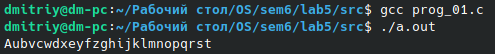
\includegraphics[scale=1.2]{inc/img/1.png}
	\caption{Программа с одним потоком}
\end{figure}

\clearpage

\listingfile{prog_01_thread.c}{prog-02-1}{C}{Открытие одного и того же файла для чтения в двух потоках}{}

\imgw{1-1}{h!}{\textwidth}{Программа с двумя потоками}

\subsection{Схема взаимодействия структур ядра}

\imgw{sch1}{h!}{\textwidth}{Схема взаимодействия структур ядра}

\subsection*{Выводы}

\begin{itemize}
	\item в результате вызова функции \texttt{open()} создается дескриптор файла в таблице открытых файлов процесса и дескриптор в системной таблице открытых файлов. В созданной структуре \texttt{struct file} хранится смещение в файле и флаги состояния файла;
	
	\item в результате двух вызовов функции \texttt{fdopen()} создаются два указателя на структуру \texttt{\_IO\_FILE}. Полю \texttt{\_fileno} присваивается значение дескриптора, который вернула функция \texttt{open()};
	
	\item функция \texttt{setvbuf()} явно задает размер буфера в 20 байт и меняет тип буферизации (для \texttt{fs1} и \texttt{fs2}) на полную;
	
	\item при первом вызове функции \texttt{fscanf()} в цикле (для \texttt{fs1}), \texttt{buff1} будет заполнен первыми 20 символами (буквами алфавита). \texttt{f\_pos} в структуре \texttt{struct file} открытого файла увеличится на 20;
	
	\item при втором вызове \texttt{fscanf()} в цикле (для \texttt{fs2}) буфер \texttt{buff2} будет заполнен оставшимися 6 символами (начиная с \texttt{f\_pos});
	
	\item в цикле поочередно выводятся символы из \texttt{buff1} и \texttt{buff2};
	
	\item в случае многопоточной реализации в потоке, который первым получит квант, первый вызов \texttt{fscanf()} заполнит буфер целиком и увеличит \texttt{f\_pos} в структуре \texttt{struct file} открытого файла, а оставшиеся 6 символов будут записаны в буфер в другом потоке.
\end{itemize}

\section{Вторая программа}

\subsection{Коды программ}

\listingfile{prog_02.c}{prog-02}{C}{Открытие одного и того же файла несколько раз для чтения в одном потоке}{}

\imgw{2}{h!}{\textwidth}{Программа с одним потоком}

\listingfile{prog_02_thread.c}{prog-02-1}{C}{Открытие одного и того же файла несколько раз для чтения в двух потоках}{}

\imgw{2-1}{h!}{\textwidth}{Программа с двумя потоками}

\clearpage

\listingfile{prog_02_mutex.c}{prog-02-2}{C}{Открытие одного и того же файла несколько раз для чтения в двух потоках с использованием мьютекса}{}

\imgw{2-2}{h!}{\textwidth}{Программа с двумя потоками и мьютексом}

\clearpage

\subsection{Схема взаимодействия структур ядра}

\imgw{sch2}{H}{1\textwidth}{Схема взаимодействия структур ядра}

\subsection*{Вывод}

\begin{itemize}
	\item в результате двух вызовов функции \texttt{open()} для одного и того же файла создаются два дескриптора в таблице открытых файлов процесса и два дескриптора в системной таблице открытых файлов, поэтому в программе существуют две различные \texttt{struct file}, но ссылающиеся на один и тот же \texttt{struct inode};
	\item из-за того что структуры \texttt{struct file} разные и значения смещения в файле независимы, посимвольная печать просто дважды выведет содержимое файла в формате <<AAbbcc...>> (в случае однопоточной реализации); 
	\item в случае многопоточной реализации потоки будут поочередно получать квант времени и печатать символы;
	\item использование мьютекса решает эту проблему: вывод второго потока начнется после окончания вывода первого потока.
\end{itemize}

\section{Третья программа}

\subsection{Коды программ}

\listingfile{prog_03.c}{prog-03}{C}{Открытие одного и того же файла несколько раз для записи в одном потоке}{}

\imgw{3}{H}{\textwidth}{Программа с одним потоком}

\clearpage

\listingfile{prog_03_thread.c}{prog-03-1}{C}{Открытие одного и того же файла несколько раз для записи в двух потоках}{}

\imgw{3-1}{H}{\textwidth}{Программа с двумя потоками}

\subsection{Схема взаимодействия структур ядра}

\imgw{sch3}{H}{1\textwidth}{Схема взаимодействия структур ядра}

\subsection*{Вывод}

\begin{itemize}
	\item файл открывается на запись два раза в результате двух вызовов функции \texttt{fopen()};
	\item функция \texttt{fprintf()} предоставляет буферизованный вывод: изначально информация пишется в буфер, а из буфера в файл, если произошло одно из событий:
		\subitem буфер полон;
		\subitem вызвана функция \texttt{fclose()};
		\subitem вызвана функция \texttt{fflush()};
	\item в данной программе информация запишется в файл в результате вызова функции \texttt{fclose()};
	\item из-за того что \texttt{f\_pos} независимы для каждого дескриптора файла, запись в файл будет производиться с его начала;
	\item таким образом, информация, записанная при первом вызове \texttt{fclose()}, будет потеряна в результате второго вызова \texttt{fclose()}.
	\item в многопоточной реализации результат аналогичен -- с помощью \texttt{pthread\_join} дожидаемся вызова \texttt{fclose()} для \texttt{f2} в отдельном потоке и далее вызываем \texttt{fclose()} для \texttt{f1}.
\end{itemize}

Для исключения проблемы потери данных нужно открывать файл в режиме добавления - \texttt{O\_APPEND}. Тогда установка смещения в конец файла и операция записи в файл выполняются как атомарная операция.